% Relatório técnico-científico (ABNT NBR 10719) com abnTeX2.
% Compilar a partir de docs/:  latexmk -pdf relatorio.tex
% As tabelas e figuras em recursos/ são geradas por:  venv/bin/python docs/gerar_recursos.py

\documentclass[
    12pt,
    oneside,
    a4paper,
    openany,
    chapter=TITLE,
    english,
    brazil
]{abntex2}

% ─── Pacotes ────────────────────────────────────────
\usepackage{cmap}
\usepackage[utf8]{inputenc}
\usepackage[T1]{fontenc}
\usepackage{lmodern}
\usepackage{indentfirst}
\usepackage{xcolor}
\usepackage{graphicx}
\usepackage{microtype}
\usepackage{booktabs}
\usepackage{siunitx}
\usepackage{amsmath}

% Ambiente "quadro" (informação textual com bordas fechadas, NBR 14724), definido
% pelo \newfloat da classe memoir antes de carregar o float, para herdar o
% estilo de legenda do abnTeX2 (título acima, separado por travessão)
% Os quadros entram na Lista de ilustrações (lof), junto com as figuras
\newfloat[chapter]{quadro}{lof}{Quadro}
\renewcommand{\thequadro}{\arabic{quadro}}
\providecommand{\quadroautorefname}{Quadro}
% O babel brazil usa "seção" minúsculo no \autoref; maiúsculo como Capítulo, Tabela etc.
\addto\captionsbrazil{%
    \renewcommand{\sectionautorefname}{Seção}%
    \renewcommand{\subsectionautorefname}{Seção}%
}
\newlistentry{quadro}{lof}{0}
\renewcommand{\cftquadroname}{Quadro\space}
\renewcommand*{\cftquadroaftersnum}{\hfill\textendash\hfill}
\setlength{\cftquadroindent}{\cftfigureindent}
\setlength{\cftquadronumwidth}{\cftfigurenumwidth}

\usepackage{float}
\usepackage{listings}
% Citações conforme a NBR 10520:2023: sobrenome só com inicial maiúscula também
% entre parênteses, ex.: (Cormen et al., 2012), e "et al." em itálico
% (a opção nbr10520-2023 está declarada no início do referencias.bib)
\usepackage[alf, nbr10520-2023, abnt-etal-text=it]{abntex2cite}
% NBR 6023:2018: URL sem os sinais < >
\def\UrlLeft{}
\def\UrlRight{}
% Autor-entidade: maiúsculas e minúsculas na citação, maiúsculas nas referências
% (o \emreferenciastrue fica logo antes do \bibliography; o comando é robusto
% para chegar sem expandir ao .aux e só decidir a caixa na hora de imprimir)
\newif\ifemreferencias
\DeclareRobustCommand{\entidade}[1]{\ifemreferencias\MakeUppercase{#1}\else#1\fi}

\sisetup{
    output-decimal-marker = {,},
    group-digits          = integer,
    group-separator       = {.},
    group-minimum-digits  = 4,
    exponent-product      = \times,
    table-number-alignment = center,
}

\lstset{
    basicstyle   = \ttfamily\footnotesize,
    frame        = single,
    breaklines   = true,
    columns      = fullflexible,
    keepspaces   = true,
    showstringspaces = false,
    inputencoding = utf8,
    extendedchars = true,
    literate = {á}{{\'a}}1 {ã}{{\~a}}1 {ç}{{\c c}}1 {é}{{\'e}}1 {ê}{{\^e}}1
               {í}{{\'i}}1 {ó}{{\'o}}1 {õ}{{\~o}}1 {ú}{{\'u}}1 {×}{{$\times$}}1,
}

% Marca itens que ainda precisam ser completados antes da entrega
\newcommand{\pendente}[1]{\textcolor{red}{\textbf{[PENDENTE: #1]}}}

% ─── Dados do trabalho ──────────────────────────────
\titulo{Análise empírica do Insertion Sort e do Merge Sort: tempos de execução, estatística descritiva e regressão polinomial}
\autor{\pendente{nome completo do aluno}}
\local{Fortaleza}
\data{2026}
\orientador{Prof. Bruno Lopes}
\instituicao{%
    Universidade de Fortaleza -- UNIFOR
    \par
    Centro de Ciências Tecnológicas
    \par
    Bacharelado em Ciência da Computação}
\tipotrabalho{Relatório técnico}
\preambulo{Relatório da atividade prática de implementação (AV2) apresentado à disciplina T198 -- Construção e Análise de Algoritmos, do curso de Bacharelado em Ciência da Computação da Universidade de Fortaleza.}

\usepackage{hyperref}
\hypersetup{
    pdftitle    = {Análise empírica do Insertion Sort e do Merge Sort},
    pdfsubject  = {Relatório técnico -- T198 Construção e Análise de Algoritmos},
    colorlinks  = true,
    linkcolor   = black,
    citecolor   = black,
    urlcolor    = black,
    bookmarksdepth = 4,
}

% NBR 14724: só o número da página, no canto superior direito
\makeevenhead{abntheadings}{}{}{\ABNTEXfontereduzida\thepage}
\makeoddhead{abntheadings}{}{}{\ABNTEXfontereduzida\thepage}
\makeheadrule{abntheadings}{\textwidth}{0pt}

\setlength{\parindent}{1.25cm}
\setlength{\parskip}{0.2cm}
% Folga extra de espaçamento, usada só quando uma linha não cabe na margem
% (ex.: caminhos em \texttt, que não esticam)
\setlength{\emergencystretch}{2em}

% ═══════════════════════════════════════════════════
\begin{document}
\selectlanguage{brazil}
\frenchspacing

% ─── PRÉ-TEXTUAIS ──────────────────────────────────
\pretextual

\imprimircapa
\imprimirfolhaderosto

\setlength{\absparsep}{18pt}
\begin{resumo}
Este relatório apresenta uma análise empírica do tempo de execução dos algoritmos de ordenação Insertion Sort e Merge Sort, implementados na linguagem C, com o objetivo de verificar se o comportamento observado na prática confirma as ordens de crescimento previstas pela análise assintótica. Os dois algoritmos foram executados sobre vetores de \num{1000} a \num{1000000} elementos em três cenários de entrada (crescente, aleatório e decrescente), com 50 repetições por combinação e medição de tempo pela função \texttt{clock\_gettime()} com o relógio \texttt{CLOCK\_MONOTONIC}. Para cada combinação foram calculados média, desvio padrão, intervalo de confiança de 95\,\%, mínimo e máximo, e foram ajustados polinômios de grau 1 a 3 às médias pelo método dos mínimos quadrados. Os resultados confirmaram o comportamento quadrático do Insertion Sort nos casos médio e pior (expoentes empíricos de 1,96 e 1,97, razão próxima de 4 ao dobrar $n$ e coeficiente de determinação de 0,999999 para o polinômio de grau 2), o comportamento linear do Insertion Sort no melhor caso e o crescimento quase linear do Merge Sort, compatível com $\Theta(n \log n)$. O Merge Sort foi significativamente mais rápido que o Insertion Sort em todos os tamanhos testados nos casos médio e pior, chegando a ser cerca de 632 vezes mais rápido com $n = \num{1000000}$ no caso médio, enquanto o Insertion Sort foi o mais rápido em todos os tamanhos do melhor caso. Conclui-se que a análise empírica confirmou as previsões teóricas e evidenciou aspectos que a notação assintótica omite, como as constantes multiplicativas e a sensibilidade de cada algoritmo à configuração da entrada.

\textbf{Palavras-chave}: algoritmos de ordenação; insertion sort; merge sort; análise empírica; regressão polinomial.
\end{resumo}

\pdfbookmark[0]{\listfigurename}{lof}
\listoffigures*
\cleardoublepage

\pdfbookmark[0]{\listtablename}{lot}
\listoftables*
\cleardoublepage

\pdfbookmark[0]{\contentsname}{toc}
\tableofcontents*
\cleardoublepage

% ─── TEXTUAIS ──────────────────────────────────────
\textual

% ═══════════════════════════════════════════════════
\chapter{Introdução}
\label{cap:introducao}

A análise assintótica descreve como o custo de um algoritmo cresce em função do tamanho da entrada, abstraindo constantes multiplicativas e termos de ordem inferior \cite{cormen2012}. Essa abstração permite comparar algoritmos independentemente de máquina, mas não informa quanto tempo um programa leva de fato para executar, nem a partir de que tamanho de entrada um algoritmo assintoticamente melhor passa a compensar na prática. Fatores como o compilador e suas otimizações, a hierarquia de memória, o sistema operacional e a própria configuração da entrada afetam o tempo real de execução. Por isso, a análise experimental é um complemento necessário à análise teórica: ela permite verificar se as previsões se confirmam e quantificar os aspectos que a notação assintótica deixa de fora \cite{johnson2002,mcgeoch2012}.

Os algoritmos de ordenação são um caso adequado para esse tipo de estudo, porque possuem análise teórica bem estabelecida e comportamento que depende fortemente da entrada. O Insertion Sort executa $\Theta(n)$ operações quando o vetor já está ordenado, mas $\Theta(n^2)$ no caso médio e no pior caso, quando o vetor está em ordem decrescente. Já o Merge Sort, baseado na estratégia de divisão e conquista, executa $\Theta(n \log n)$ operações em qualquer caso, ao custo de memória auxiliar proporcional a $n$ \cite{cormen2012}.

O objetivo deste trabalho foi implementar os dois algoritmos na linguagem C, medir seus tempos de execução para dez tamanhos de entrada, entre \num{1000} e \num{1000000} elementos, em três cenários (melhor caso, caso médio e pior caso), e analisar os dados por meio de estatística descritiva e regressão polinomial. Com base na teoria, esperava-se observar que:

\begin{alineas}
    \item o tempo do Insertion Sort cresce de forma aproximadamente quadrática nos casos médio e pior, multiplicando-se por cerca de 4 a cada vez que $n$ dobra, e de forma linear no melhor caso;
    \item o tempo do Merge Sort cresce de forma ligeiramente superior à linear em todos os cenários, multiplicando-se por pouco mais de 2 quando $n$ dobra;
    \item o Merge Sort supera o Insertion Sort nos casos médio e pior a partir de algum tamanho de entrada, com a diferença aumentando rapidamente com $n$, enquanto no melhor caso o Insertion Sort permanece mais rápido;
    \item o polinômio de grau 2 se ajusta bem aos dados do Insertion Sort nos casos médio e pior.
\end{alineas}

O \autoref{cap:metodologia} descreve o ambiente e o procedimento experimental. O \autoref{cap:resultados} apresenta os dados coletados, sem interpretação. O \autoref{cap:analise} interpreta os resultados à luz da teoria, incluindo a regressão polinomial, e o \autoref{cap:conclusao} sintetiza as conclusões.

% ═══════════════════════════════════════════════════
\chapter{Metodologia}
\label{cap:metodologia}

Este capítulo descreve o ambiente de execução, a implementação, a geração das entradas, a coleta dos dados e os métodos estatísticos empregados, com o detalhamento necessário para que o experimento possa ser reproduzido. O \autoref{apendice:reproducao} lista os comandos utilizados.

\section{Ambiente de execução}

Os experimentos foram executados em um computador com as especificações do \autoref{quadro:ambiente}.

\begin{quadro}[htbp]
    \caption{Especificações do ambiente de execução}
    \label{quadro:ambiente}
    \centering
    \small
    \begin{tabular}{|l|p{9.5cm}|}
        \hline
        \textbf{Item} & \textbf{Especificação} \\ \hline
        Processador & Intel Core i5-12400 (12.ª geração), 6 núcleos e 12 \textit{threads}, cache L2 de 7,5 MiB e L3 de 18 MiB \\ \hline
        Memória RAM & 15,5 GiB disponíveis para a máquina virtual do WSL 2; \pendente{informar a RAM física total do computador} \\ \hline
        Sistema hospedeiro & Microsoft Windows 11 (versão 10.0.26200) \\ \hline
        Sistema de execução & Ubuntu 26.04.1 LTS no Windows Subsystem for Linux 2 (WSL 2), núcleo Linux 6.18.33.2-microsoft-standard-WSL2 \\ \hline
        Compilador & GCC 15.2.0 \\ \hline
        Flags de compilação & \texttt{-Wall -Wextra -O2} \\ \hline
        Análise de dados & Python 3.14.4 com NumPy 2.5.3, pandas 3.0.6, SciPy 1.18.1 e Matplotlib 3.11.2 \\ \hline
    \end{tabular}
    \fonte{Elaborado pelo autor (2026).}
\end{quadro}

O programa foi compilado pelo \texttt{Makefile} do projeto com o comando \texttt{gcc -Wall -Wextra -O2 main.c sorts.c -o main}. As opções \texttt{-Wall} e \texttt{-Wextra} apenas habilitam avisos do compilador e não alteram o código gerado. A opção \texttt{-O2} habilita o conjunto de otimizações do GCC que não envolvem uma troca entre espaço e velocidade \cite{gcc2025}. Ela foi escolhida porque representa a forma como programas em C costumam ser compilados para uso real. As otimizações reduzem as constantes multiplicativas do tempo de execução, mas não alteram o número de comparações e movimentações que cada algoritmo realiza; portanto, não alteram a ordem de crescimento. Os tempos absolutos seriam outros com \texttt{-O0} ou \texttt{-O3}, mas as razões entre tamanhos de entrada e os expoentes analisados no \autoref{cap:analise} devem se manter.

Durante as execuções, o computador foi utilizado normalmente, sem isolamento de núcleos de processamento nem desativação do ajuste dinâmico de frequência do processador. Esses fatores, somados à camada de virtualização do WSL 2, são fontes de variação entre as repetições e foram considerados na análise da variabilidade (\autoref{sec:variabilidade}).

\section{Implementação dos algoritmos}

Os algoritmos foram implementados no arquivo \texttt{sorts.c}, com base nos pseudocódigos de \citeonline{cormen2012}, ambos ordenando vetores de inteiros (\texttt{int}) em ordem crescente:

\begin{alineas}
    \item \textbf{Insertion Sort} (\texttt{insertion\_sort}): percorre o vetor da segunda posição em diante; cada elemento é guardado em uma variável auxiliar (\texttt{chave}) e os elementos maiores à sua esquerda são deslocados uma posição para a direita até que a posição correta seja encontrada. A ordenação é feita no próprio vetor, sem memória adicional;
    \item \textbf{Merge Sort} (\texttt{merge\_sort}): versão recursiva descendente, que divide o intervalo $[p, r]$ ao meio, ordena cada metade recursivamente e intercala as duas metades com a função \texttt{merge}. Cada chamada de \texttt{merge} aloca com \texttt{malloc} dois vetores auxiliares, com as cópias das duas metades, e os libera com \texttt{free} ao final; o custo dessas alocações faz parte do tempo medido. A função \texttt{merge\_sort\_wrapper(v, n)} adapta a assinatura para \texttt{(int v[], int n)}, igual à do Insertion Sort, o que permite medir os dois algoritmos com a mesma função.
\end{alineas}

\section{Medição do tempo}

O tempo foi medido pela função \texttt{medir}, do arquivo \texttt{main.c}, que recebe um ponteiro para a função de ordenação, chama \texttt{clock\_gettime(CLOCK\_MONOTONIC, ...)} imediatamente antes e imediatamente depois da ordenação e devolve a diferença em segundos, com resolução de nanossegundos. Apenas a chamada da ordenação fica entre as duas leituras do relógio; a geração do vetor e a gravação em arquivo ficam fora do intervalo medido.

O relógio \texttt{CLOCK\_MONOTONIC} foi escolhido porque mede o tempo decorrido a partir de um ponto fixo e não sofre os saltos que afetam o relógio de tempo real do sistema (\texttt{CLOCK\_REALTIME}), como ajustes manuais da hora ou sincronizações automáticas \cite{manclock}. Ele também oferece resolução muito superior à da função \texttt{clock()} da biblioteca padrão, que mede o tempo de processador em unidades de \texttt{CLOCKS\_PER\_SEC}. Por medir o tempo decorrido, e não apenas o tempo de processador, o valor obtido inclui eventuais interrupções do processo pelo sistema operacional, o que contribui para a variabilidade observada.

\section{Geração das entradas}
\label{sec:entradas}

Para cada cenário, o vetor foi preenchido pela função \texttt{preencher}, que seleciona uma das funções a seguir:

\begin{alineas}
    \item \textbf{melhor caso} (\texttt{preencher\_crescente}): valores de 1 a $n$ em ordem crescente (\texttt{v[k] = k + 1}). Para o Insertion Sort é o melhor caso, pois nenhum elemento precisa ser deslocado;
    \item \textbf{caso médio} (\texttt{preencher\_aleatorio}): valores gerados pela função \texttt{rand()} da biblioteca padrão, no intervalo de 0 a \texttt{RAND\_MAX} ($2^{31} - 1$ na biblioteca GNU C). Antes de cada preenchimento, o gerador é inicializado com \texttt{srand(j + 1)}, em que $j$ é o índice da repetição, de 0 a 49. Assim, cada uma das 50 repetições usa um vetor aleatório diferente, como exige o enunciado;
    \item \textbf{pior caso} (\texttt{preencher\_decrescente}): valores de $n$ a 1 em ordem decrescente (\texttt{v[k] = n - k}). Para o Insertion Sort é o pior caso, pois cada elemento precisa ser deslocado até o início do vetor.
\end{alineas}

Para garantir que os dois algoritmos ordenassem exatamente o mesmo vetor em cada teste, o vetor foi gerado novamente, de forma determinística, imediatamente antes de cada execução, e não apenas uma vez. Nos cenários crescente e decrescente o conteúdo depende somente de $n$. No caso médio, como o gerador é reinicializado com a mesma semente (\texttt{srand(j + 1)}) antes da repetição $j$ de cada algoritmo, a sequência de números produzida por \texttt{rand()} é idêntica. Dessa forma, a repetição $j$ do Insertion Sort e a repetição $j$ do Merge Sort recebem vetores com conteúdo idêntico, o que tem o mesmo efeito de gerar o vetor uma vez e copiá-lo para cada algoritmo. A regeneração também é necessária porque a ordenação é feita no próprio vetor: sem ela, o segundo algoritmo receberia um vetor já ordenado.

\section{Coleta e organização dos dados}

Para cada combinação de algoritmo, cenário e tamanho $n \in \{\num{1000},\allowbreak \num{2000},\allowbreak \num{5000},\allowbreak \num{10000},\allowbreak \num{20000},\allowbreak \num{50000},\allowbreak \num{100000},\allowbreak \num{200000},\allowbreak \num{500000},\allowbreak \num{1000000}\}$, foram realizadas 50 repetições consecutivas. O laço principal percorre os cenários, depois os tamanhos e, para cada tamanho, executa as 50 repetições de um algoritmo e em seguida as 50 do outro, reaproveitando um único vetor alocado por tamanho. O bloco de configuração no início do \texttt{main.c} permite selecionar quais algoritmos, cenários e tamanhos executar, o que permitiu realizar a coleta em várias execuções, entre 21 e 22 de outubro de 2026.

Cada combinação gera um arquivo CSV próprio, no caminho \texttt{resultados/\allowbreak<algoritmo>/\allowbreak<cenário>/\allowbreak<n>.csv}, por exemplo \texttt{resultados/\allowbreak merge/\allowbreak medio/\allowbreak 0100000.csv}. Cada arquivo tem um cabeçalho e uma linha por repetição, com os campos \texttt{algoritmo}, \texttt{cenario}, \texttt{n}, \texttt{repeticao} e \texttt{tempo\_s}.

Até a redação desta versão do relatório, duas combinações estavam incompletas: o arquivo do Insertion Sort no caso médio com $n = \num{100000}$ registra 46 das 50 repetições, devido a uma execução interrompida; e o pior caso com $n = \num{1000000}$ ainda não havia sido executado para nenhum dos algoritmos. \pendente{completar as 50 repetições do Insertion Sort no caso médio com $n = \num{100000}$ e executar o pior caso com $n = \num{1000000}$; depois, gerar os recursos novamente e revisar os trechos marcados nos capítulos \ref{cap:resultados}, \ref{cap:analise} e \ref{cap:conclusao}}

\section{Estatística descritiva}
\label{sec:estatistica}

O processamento dos dados foi feito em Python, com as bibliotecas pandas \cite{mckinney2010}, NumPy \cite{harris2020}, SciPy \cite{virtanen2020} e Matplotlib \cite{hunter2007}, pelos programas \texttt{analise.py} e \texttt{docs/gerar\_recursos.py} do projeto. Para cada combinação, com $r$ repetições e tempos $t_1, \ldots, t_r$, foram calculados a média $\bar{t}$, o desvio padrão amostral $s$, os valores mínimo e máximo e o intervalo de confiança de 95\,\% para a média, dado pela \autoref{eq:ic}. A equação usa a distribuição $t$ de Student, que, segundo \citeonline{montgomery2016}, é a adequada quando a variância populacional é desconhecida:

\begin{equation}
    \label{eq:ic}
    \bar{t} \pm t_{0{,}975;\,r-1} \cdot \frac{s}{\sqrt{r}}
\end{equation}

Com $r = 50$ repetições, o quantil é $t_{0{,}975;\,49} \approx 2{,}0096$. O intervalo indica a faixa em que se espera encontrar o tempo médio verdadeiro da combinação, com 95\,\% de confiança.

Para decidir se a diferença entre os dois algoritmos é significativa em um dado $n$, foram usados dois critérios em conjunto: a ausência de sobreposição entre os intervalos de confiança das duas médias e o teste $t$ de Welch, que compara duas médias sem supor variâncias iguais \cite{welch1947}, com nível de significância $\alpha = 0{,}05$.

\section{Regressão polinomial e indicadores de crescimento}
\label{sec:metodo-regressao}

Para cada combinação de algoritmo e cenário, foram ajustados polinômios de grau 1, 2 e 3 às médias de tempo em função de $n$ (dez pontos por combinação), pelo método dos mínimos quadrados, com a função \texttt{numpy.polyfit} \cite{harris2020}. Para evitar problemas numéricos com potências muito grandes de $n$, o ajuste foi feito sobre a variável $x = n / 10^6$, e os coeficientes foram depois convertidos para a variável $n$. A qualidade de cada ajuste foi medida pelo coeficiente de determinação $R^2$. Como a função teórica do Merge Sort não é polinomial, foi ajustado também, para comparação, o modelo $T(n) = a \, n \log_2 n + b$, pelo mesmo método.

Foram calculados ainda dois indicadores complementares:

\begin{alineas}
    \item \textbf{razão ao dobrar $n$}: $T(2n)/T(n)$ para os pares de tamanhos em que $2n$ também foi medido. Se $T(n) \propto n^k$, essa razão vale $2^k$: 2 para crescimento linear e 4 para crescimento quadrático. Para $T(n) \propto n \log_2 n$, vale $2 \log_2(2n) / \log_2 n$, ou seja, entre 2,10 e 2,20 no intervalo estudado;
    \item \textbf{expoente empírico $k$}: inclinação da reta ajustada por mínimos quadrados aos pontos $(\log n, \log T)$. Se $T(n) \propto n^k$, os pontos ficam sobre uma reta de inclinação $k$.
\end{alineas}

% ═══════════════════════════════════════════════════
\chapter{Resultados}
\label{cap:resultados}

Este capítulo apresenta os dados coletados, sem interpretação. As tabelas \ref{tab:est-insertion-melhor} a \ref{tab:est-merge-pior} trazem as estatísticas de cada combinação de algoritmo, cenário e tamanho de entrada, com todos os tempos em milissegundos. A coluna \emph{Rep.} indica o número de repetições válidas.

\section{Estatísticas do Insertion Sort}

\begin{table}[H]
    \caption{Insertion Sort, melhor caso: estatísticas do tempo de execução (ms)}
    \label{tab:est-insertion-melhor}
    \centering
    \small
    \begin{tabular}{r S[table-format=1.7] S[table-format=1.8] S[table-format=1.8] S[table-format=1.7] S[table-format=1.6] r}
\toprule
{$n$} & {Média} & {Desvio padrão} & {IC 95\,\% ($\pm$)} & {Mínimo} & {Máximo} & {Rep.} \\
\midrule
1.000 & 0.0007371 & 0.00007556 & 0.00002147 & 0.0007100 & 0.001222 & 50 \\
2.000 & 0.001844 & 0.0003830 & 0.0001088 & 0.001370 & 0.002513 & 50 \\
5.000 & 0.005648 & 0.002054 & 0.0005839 & 0.003382 & 0.01606 & 50 \\
10.000 & 0.01531 & 0.01081 & 0.003071 & 0.006737 & 0.06108 & 50 \\
20.000 & 0.01799 & 0.004085 & 0.001161 & 0.01341 & 0.03736 & 50 \\
50.000 & 0.04089 & 0.007348 & 0.002088 & 0.03352 & 0.05854 & 50 \\
100.000 & 0.1161 & 0.03471 & 0.009866 & 0.06902 & 0.2265 & 50 \\
200.000 & 0.1542 & 0.03028 & 0.008605 & 0.1338 & 0.2525 & 50 \\
500.000 & 0.4660 & 0.1307 & 0.03715 & 0.3345 & 0.7889 & 50 \\
1.000.000 & 0.8295 & 0.1872 & 0.05319 & 0.6718 & 1.316 & 50 \\
\bottomrule
\end{tabular}

    \fonte{Elaborada pelo autor (2026).}
\end{table}

\begin{table}[H]
    \caption{Insertion Sort, caso médio: estatísticas do tempo de execução (ms)}
    \label{tab:est-insertion-medio}
    \centering
    \small
    \begin{tabular}{r S[table-format=5.5] S[table-format=3.5] S[table-format=3.6] S[table-format=5.5] S[table-format=5.4] r}
\toprule
{$n$} & {Média} & {Desvio padrão} & {IC 95\,\% ($\pm$)} & {Mínimo} & {Máximo} & {Rep.} \\
\midrule
1.000 & 0.09701 & 0.01541 & 0.004380 & 0.07151 & 0.1399 & 50 \\
2.000 & 0.3420 & 0.1189 & 0.03378 & 0.2686 & 0.9552 & 50 \\
5.000 & 1.690 & 0.1051 & 0.02988 & 1.605 & 2.162 & 50 \\
10.000 & 7.049 & 1.096 & 0.3116 & 6.377 & 11.01 & 50 \\
20.000 & 27.23 & 1.667 & 0.4737 & 25.56 & 33.48 & 50 \\
50.000 & 172.2 & 6.569 & 1.867 & 161.9 & 192.6 & 50 \\
100.000 & 673.8 & 12.65 & 3.596 & 656.7 & 718.2 & 50 \\
200.000 & 2698 & 31.29 & 8.891 & 2648 & 2801 & 50 \\
500.000 & 16856 & 198.4 & 56.39 & 16551 & 17864 & 50 \\
1.000.000 & 66828 & 665.0 & 189.0 & 65699 & 69661 & 50 \\
\bottomrule
\end{tabular}

    \fonte{Elaborada pelo autor (2026).}
\end{table}

\begin{table}[H]
    \caption{Insertion Sort, pior caso: estatísticas do tempo de execução (ms)}
    \label{tab:est-insertion-pior}
    \centering
    \small
    \begin{tabular}{r S[table-format=6.4] S[table-format=4.5] S[table-format=3.6] S[table-format=6.4] S[table-format=6.4] r}
\toprule
{$n$} & {Média} & {Desvio padrão} & {IC 95\,\% ($\pm$)} & {Mínimo} & {Máximo} & {Rep.} \\
\midrule
1.000 & 0.1536 & 0.02128 & 0.006047 & 0.1344 & 0.2009 & 50 \\
2.000 & 0.5419 & 0.04133 & 0.01175 & 0.5197 & 0.7560 & 50 \\
5.000 & 3.561 & 0.4619 & 0.1313 & 3.191 & 5.203 & 50 \\
10.000 & 13.70 & 0.9384 & 0.2667 & 12.82 & 18.24 & 50 \\
20.000 & 56.60 & 3.111 & 0.8842 & 52.27 & 64.37 & 50 \\
50.000 & 344.0 & 6.694 & 1.902 & 331.5 & 357.0 & 50 \\
100.000 & 1419 & 67.37 & 19.15 & 1341 & 1651 & 50 \\
200.000 & 5702 & 245.7 & 69.83 & 5398 & 6468 & 50 \\
500.000 & 34049 & 1131 & 321.5 & 32779 & 36963 & 50 \\
1.000.000 & 133541 & 1885 & 535.7 & 131812 & 144296 & 50 \\
\bottomrule
\end{tabular}

    \fonte{Elaborada pelo autor (2026).}
\end{table}

\section{Estatísticas do Merge Sort}

\begin{table}[H]
    \caption{Merge Sort, melhor caso: estatísticas do tempo de execução (ms)}
    \label{tab:est-merge-melhor}
    \centering
    \small
    \begin{tabular}{r S[table-format=2.5] S[table-format=1.6] S[table-format=1.6] S[table-format=2.5] S[table-format=2.5] r}
\toprule
{$n$} & {Média} & {\cabecalho{Desvio\\padrão}} & {\cabecalho{IC 95\,\%\\($\pm$)}} & {Mínimo} & {Máximo} & {Rep.} \\
\midrule
1.000 & 0.02718 & 0.004353 & 0.001237 & 0.02197 & 0.03746 & 50 \\
2.000 & 0.05381 & 0.006466 & 0.001838 & 0.04699 & 0.07788 & 50 \\
5.000 & 0.1553 & 0.02699 & 0.007670 & 0.1200 & 0.2443 & 50 \\
10.000 & 0.2592 & 0.01848 & 0.005252 & 0.2414 & 0.3109 & 50 \\
20.000 & 0.5038 & 0.01620 & 0.004605 & 0.4875 & 0.5793 & 50 \\
50.000 & 1.395 & 0.1898 & 0.05393 & 1.242 & 2.383 & 50 \\
100.000 & 2.820 & 0.3414 & 0.09703 & 2.575 & 3.933 & 50 \\
200.000 & 5.979 & 0.7643 & 0.2172 & 5.266 & 8.522 & 50 \\
500.000 & 15.57 & 1.484 & 0.4217 & 13.80 & 19.67 & 50 \\
1.000.000 & 31.92 & 3.530 & 1.003 & 27.96 & 49.70 & 50 \\
\bottomrule
\end{tabular}

    \fonte{Elaborada pelo autor (2026).}
\end{table}

\begin{table}[H]
    \caption{Merge Sort, caso médio: estatísticas do tempo de execução (ms)}
    \label{tab:est-merge-medio}
    \centering
    \small
    \begin{tabular}{r S[table-format=3.5] S[table-format=1.6] S[table-format=1.6] S[table-format=3.5] S[table-format=3.4] r}
\toprule
{$n$} & {Média} & {\cabecalho{Desvio\\padrão}} & {\cabecalho{IC 95\,\%\\($\pm$)}} & {Mínimo} & {Máximo} & {Rep.} \\
\midrule
1.000 & 0.07454 & 0.009176 & 0.002608 & 0.05847 & 0.1105 & 50 \\
2.000 & 0.1291 & 0.005195 & 0.001476 & 0.1230 & 0.1460 & 50 \\
5.000 & 0.3806 & 0.05492 & 0.01561 & 0.3317 & 0.5769 & 50 \\
10.000 & 0.7936 & 0.2022 & 0.05745 & 0.7009 & 1.979 & 50 \\
20.000 & 1.627 & 0.1331 & 0.03783 & 1.499 & 1.980 & 50 \\
50.000 & 4.381 & 1.161 & 0.3299 & 4.043 & 12.37 & 50 \\
100.000 & 9.222 & 0.9726 & 0.2764 & 8.534 & 14.49 & 50 \\
200.000 & 19.86 & 2.046 & 0.5815 & 18.22 & 30.77 & 50 \\
500.000 & 51.78 & 2.631 & 0.7478 & 48.46 & 60.76 & 50 \\
1.000.000 & 105.7 & 2.482 & 0.7055 & 102.6 & 115.2 & 50 \\
\bottomrule
\end{tabular}

    \fonte{Elaborada pelo autor (2026).}
\end{table}

\begin{table}[H]
    \caption{Merge Sort, pior caso: estatísticas do tempo de execução (ms)}
    \label{tab:est-merge-pior}
    \centering
    \small
    \begin{tabular}{r S[table-format=2.5] S[table-format=1.6] S[table-format=1.6] S[table-format=2.5] S[table-format=2.5] r}
\toprule
{$n$} & {Média} & {Desvio padrão} & {IC 95\,\% ($\pm$)} & {Mínimo} & {Máximo} & {Rep.} \\
\midrule
1.000 & 0.03045 & 0.005841 & 0.001660 & 0.02209 & 0.04731 & 50 \\
2.000 & 0.05391 & 0.005349 & 0.001520 & 0.05074 & 0.08876 & 50 \\
5.000 & 0.1317 & 0.01193 & 0.003391 & 0.1171 & 0.1703 & 50 \\
10.000 & 0.2903 & 0.04193 & 0.01192 & 0.2387 & 0.4350 & 50 \\
20.000 & 0.5615 & 0.07505 & 0.02133 & 0.4922 & 0.8384 & 50 \\
50.000 & 1.447 & 0.1725 & 0.04901 & 1.259 & 1.931 & 50 \\
100.000 & 2.820 & 0.7947 & 0.2258 & 2.582 & 8.200 & 50 \\
200.000 & 6.019 & 1.581 & 0.4494 & 5.288 & 13.25 & 50 \\
500.000 & 14.92 & 1.325 & 0.3767 & 13.78 & 19.25 & 50 \\
\bottomrule
\end{tabular}

    \fonte{Elaborada pelo autor (2026).}
\end{table}

\section{Gráficos comparativos}

As figuras \ref{fig:comp-melhor} a \ref{fig:comp-pior} mostram, para cada cenário, o tempo médio de execução de cada algoritmo em função de $n$, com barras de erro correspondentes ao intervalo de confiança de 95\,\%. Como os tempos variam ao longo de até seis ordens de grandeza, o eixo vertical está em escala logarítmica.

\begin{figure}[H]
    \caption{Tempo médio de execução no melhor caso (vetor crescente)}
    \label{fig:comp-melhor}
    \centering
    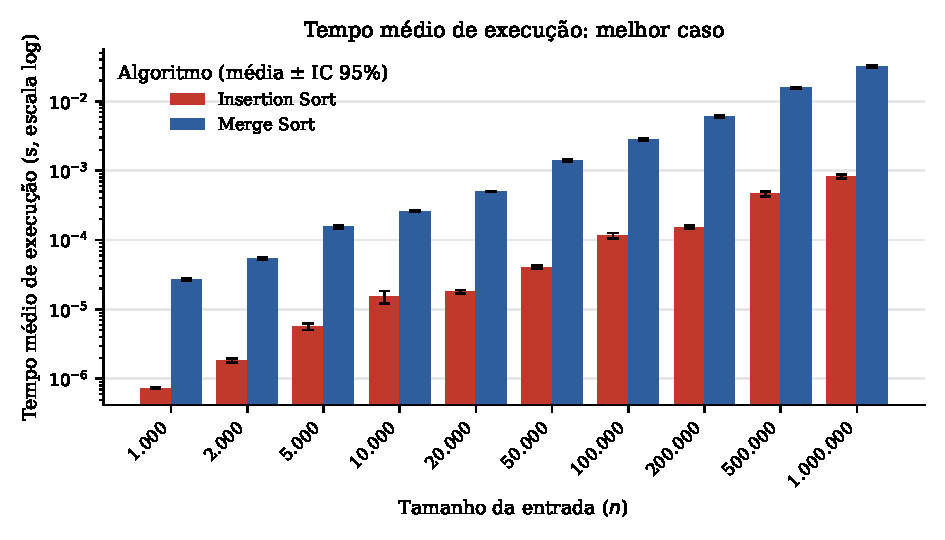
\includegraphics[width=\textwidth]{recursos/figuras/comparativo_melhor.pdf}
    \fonte{Elaborada pelo autor (2026).}
\end{figure}

\begin{figure}[H]
    \caption{Tempo médio de execução no caso médio (vetor aleatório)}
    \label{fig:comp-medio}
    \centering
    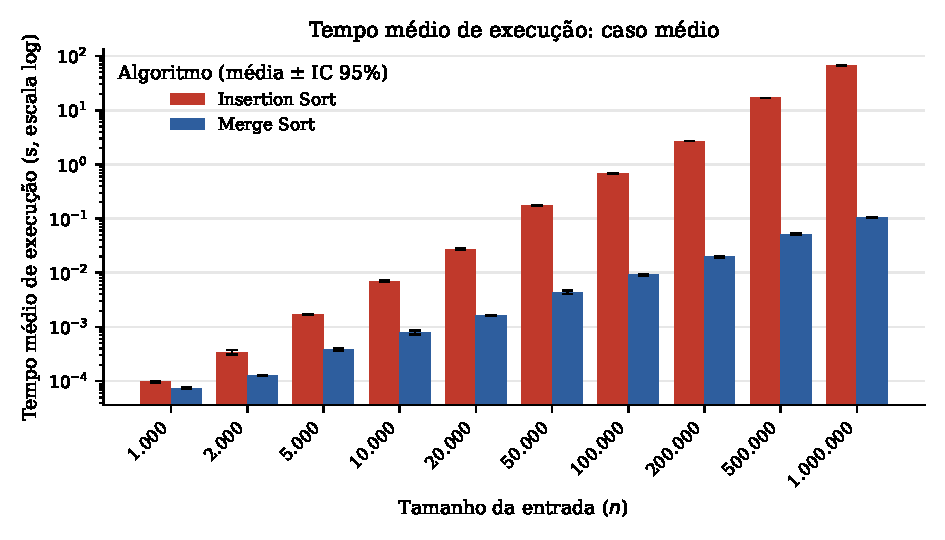
\includegraphics[width=\textwidth]{recursos/figuras/comparativo_medio.pdf}
    \fonte{Elaborada pelo autor (2026).}
\end{figure}

\begin{figure}[H]
    \caption{Tempo médio de execução no pior caso (vetor decrescente)}
    \label{fig:comp-pior}
    \centering
    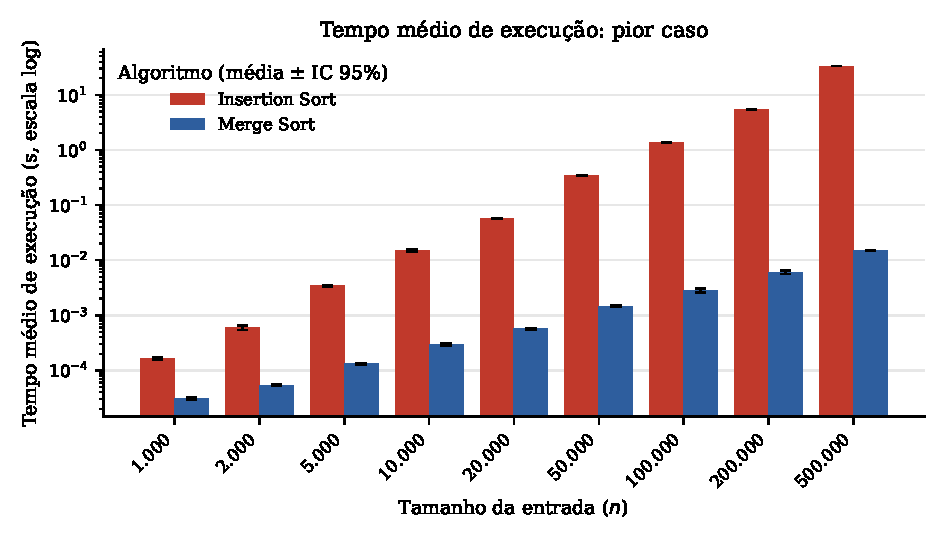
\includegraphics[width=\textwidth]{recursos/figuras/comparativo_pior.pdf}
    \fonte{Elaborada pelo autor (2026).}
\end{figure}

\pendente{a \autoref{fig:comp-pior} e as tabelas \ref{tab:est-insertion-pior} e \ref{tab:est-merge-pior} ainda não incluem $n = \num{1000000}$}

% ═══════════════════════════════════════════════════
\chapter{Análise}
\label{cap:analise}

Este capítulo interpreta os resultados do \autoref{cap:resultados} à luz da análise teórica dos algoritmos, respondendo às questões propostas no enunciado. As análises do pior caso consideram os tamanhos de \num{1000} a \num{500000}.

\section{Ordens de crescimento observadas}
\label{sec:ordens}

Nos gráficos comparativos, a diferença de comportamento entre os algoritmos é visível pela inclinação das barras. Como o eixo vertical é logarítmico, uma mesma razão de crescimento aparece como um mesmo degrau de altura. Nos casos médio e pior (figuras \ref{fig:comp-medio} e \ref{fig:comp-pior}), as barras do Insertion Sort sobem muito mais rápido que as do Merge Sort. No caso médio, o tempo do Insertion Sort passa de 0,097\,ms com $n = \num{1000}$ para \num{66828}\,ms (cerca de 67 segundos) com $n = \num{1000000}$, um aumento de aproximadamente $6{,}9 \times 10^5$ vezes para um aumento de $10^3$ vezes em $n$, compatível com crescimento quadrático ($10^{3 \cdot 2} = 10^6$). No mesmo intervalo, o tempo do Merge Sort passa de 0,075\,ms para 105,7\,ms, um aumento de cerca de \num{1400} vezes, pouco acima do aumento linear de $10^3$ vezes, como esperado de $n \log n$.

A \autoref{fig:loglog} reúne as seis séries em escala log-log, na qual uma função $T(n) \propto n^k$ aparece como uma reta de inclinação $k$. A \autoref{tab:expoentes} apresenta essas inclinações, os expoentes empíricos.

\begin{figure}[H]
    \caption{Tempo médio em função de $n$ em escala log-log}
    \label{fig:loglog}
    \centering
    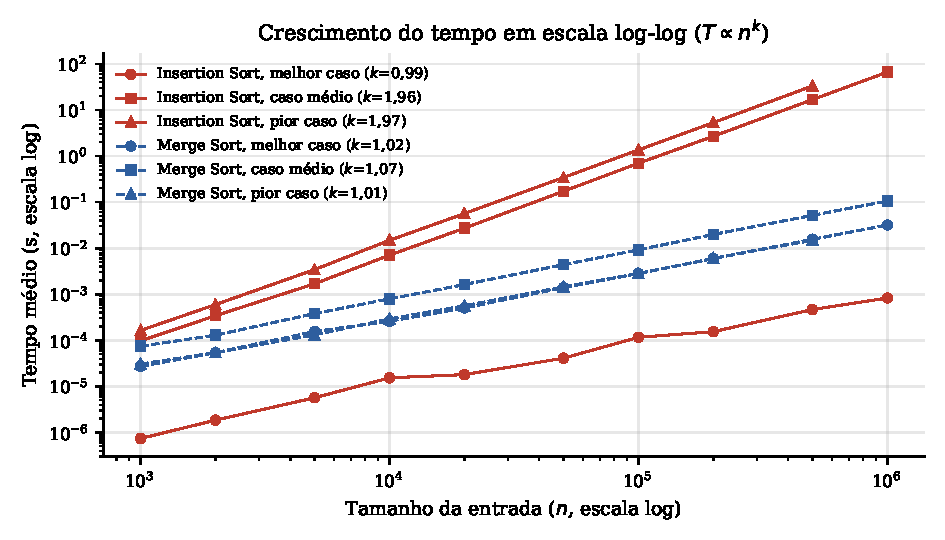
\includegraphics[width=\textwidth]{recursos/figuras/loglog.pdf}
    \fonte{Elaborada pelo autor (2026).}
\end{figure}

\begin{table}[H]
    \caption{Expoentes empíricos $k$, obtidos pela inclinação no gráfico log-log}
    \label{tab:expoentes}
    \centering
    \small
    \begin{tabular}{l l S[table-format=1.3] l}
\toprule
Algoritmo & Cenário & {Expoente $k$} & Expoente esperado \\
\midrule
Insertion Sort & Melhor caso & 0.987 & 1 ($\Theta(n)$) \\
Insertion Sort & Caso médio & 1.960 & 2 ($\Theta(n^2)$) \\
Insertion Sort & Pior caso & 1.973 & 2 ($\Theta(n^2)$) \\
Merge Sort & Melhor caso & 1.021 & $\approx 1{,}10$ ($\Theta(n \log n)$) \\
Merge Sort & Caso médio & 1.066 & $\approx 1{,}10$ ($\Theta(n \log n)$) \\
Merge Sort & Pior caso & 1.008 & $\approx 1{,}10$ ($\Theta(n \log n)$) \\
\bottomrule
\end{tabular}

    \fonte{Elaborada pelo autor (2026).}
\end{table}

Os expoentes do Insertion Sort nos casos médio (1,960) e pior (1,973) são muito próximos de 2, e o do melhor caso (0,987) é muito próximo de 1, confirmando que o algoritmo é $\Theta(n^2)$ nos dois primeiros cenários e $\Theta(n)$ no último \cite{cormen2012}. A ligeira diferença em relação a 2 se explica pelos termos de ordem inferior, que pesam relativamente mais nos menores valores de $n$.

Para o Merge Sort, os expoentes ficaram entre 1,008 e 1,066, abaixo do valor de aproximadamente 1,10 que uma função exatamente proporcional a $n \log_2 n$ teria nesse intervalo. A diferença é pequena e indica que, nos menores tamanhos, custos que não crescem com $n \log n$, como as chamadas de função e as alocações de memória, pesam proporcionalmente mais e achatam a inclinação. Ainda assim, o crescimento é claramente muito inferior ao quadrático e compatível com $\Theta(n \log n)$. Como o fator $\log_2 n$ varia apenas de cerca de 10 para cerca de 20 em todo o intervalo estudado, distinguir com precisão $n \log n$ de $n$ exigiria tamanhos de entrada ainda maiores.

\section{Comportamento ao dobrar o tamanho da entrada}
\label{sec:dobro}

A \autoref{tab:razao} mostra a razão $T(2n)/T(n)$ para os seis pares de tamanhos em que o dobro de $n$ foi medido, ao lado da razão esperada pela teoria.

\begin{table}[H]
    \caption{Razão $T(2n)/T(n)$ entre os tempos médios ao dobrar $n$}
    \label{tab:razao}
    \centering
    \small
    \begin{tabular}{l S[table-format=1.2] S[table-format=1.2] S[table-format=1.2] S[table-format=1.2] S[table-format=1.2] S[table-format=1.2] }
\toprule
 & \multicolumn{3}{c}{Insertion Sort} & \multicolumn{3}{c}{Merge Sort} \\
\cmidrule(lr){2-4}\cmidrule(lr){5-7}
{$n \to 2n$} & {Melhor caso} & {Caso médio} & {Pior caso} & {Melhor caso} & {Caso médio} & {Pior caso} \\
\midrule
1.000 $\to$ 2.000 & 2.50 & 3.53 & 3.65 & 1.98 & 1.73 & 1.77 \\
5.000 $\to$ 10.000 & 2.71 & 4.17 & 4.33 & 1.67 & 2.09 & 2.20 \\
10.000 $\to$ 20.000 & 1.18 & 3.86 & 3.81 & 1.94 & 2.05 & 1.93 \\
50.000 $\to$ 100.000 & 2.84 & 4.07 & 3.97 & 2.02 & 2.11 & 1.95 \\
100.000 $\to$ 200.000 & 1.33 & 3.85 & 3.92 & 2.12 & 2.15 & 2.13 \\
500.000 $\to$ 1.000.000 & 1.78 & 3.96 & {--} & 2.05 & 2.04 & {--} \\
\midrule
Esperada (teoria) & 2.0 & 4.0 & 4.0 & {$\approx 2{,}1$} & {$\approx 2{,}1$} & {$\approx 2{,}1$} \\
\bottomrule
\end{tabular}

    \fonte{Elaborada pelo autor (2026).}
\end{table}

No Insertion Sort, nos casos médio e pior, as razões ficaram entre 3,53 e 4,33, oscilando em torno de 4, o valor esperado para um algoritmo quadrático: dobrar a entrada quadruplica o tempo, porque o número de deslocamentos é proporcional ao número de inversões do vetor, que é da ordem de $n^2$ \cite{knuth1998}. Os valores mais afastados de 4 ocorreram nos menores tamanhos ($\num{1000} \to \num{2000}$), em que os tempos são inferiores a 1\,ms e mais sensíveis a ruído e a efeitos de cache. Do par $\num{5000} \to \num{10000}$ em diante, todas as razões ficaram entre 3,81 e 4,33.

No melhor caso, as razões do Insertion Sort variaram bastante (de 1,18 a 2,84), embora em torno de 2, o valor esperado para crescimento linear. Essa irregularidade não contradiz a teoria: nesse cenário os tempos são da ordem de microssegundos (menos de 1\,ms mesmo com um milhão de elementos), de modo que pequenas perturbações do sistema têm grande efeito relativo, como mostra a \autoref{sec:variabilidade}.

No Merge Sort, as razões ficaram entre 1,67 e 2,20 nos três cenários. A partir do par $\num{50000} \to \num{100000}$, todas ficaram entre 1,95 e 2,15, próximas do valor esperado, de aproximadamente 2,1. A razão ligeiramente superior a 2 é a assinatura do fator logarítmico: dobrar $n$ dobra o trabalho de cada nível de intercalação e acrescenta um nível à recursão.

\pendente{incluir na análise o par $\num{500000} \to \num{1000000}$ do pior caso}

\section{Comparação entre os algoritmos}
\label{sec:comparacao}

As tabelas \ref{tab:comp-melhor} a \ref{tab:comp-pior} comparam os tempos médios dos dois algoritmos em cada tamanho, com a razão entre eles (Insertion/Merge) e os resultados dos dois critérios de significância descritos na \autoref{sec:estatistica}.

\begin{table}[H]
    \caption{Comparação entre os algoritmos no melhor caso}
    \label{tab:comp-melhor}
    \centering
    \small
    \begin{tabular}{r S[table-format=1.7] S[table-format=2.5] S[table-format=1.4] c c}
\toprule
{$n$} & {\cabecalho{Insertion\\(ms)}} & {\cabecalho{Merge\\(ms)}} & {\cabecalho{Razão\\I/M}} & \cabecalho{IC se\\sobrepõem?} & \cabecalho{Diferença\\significativa?} \\
\midrule
1.000 & 0.0007371 & 0.02718 & 0.0271 & Não & Sim \\
2.000 & 0.001844 & 0.05381 & 0.0343 & Não & Sim \\
5.000 & 0.005648 & 0.1553 & 0.0364 & Não & Sim \\
10.000 & 0.01531 & 0.2592 & 0.0591 & Não & Sim \\
20.000 & 0.01799 & 0.5038 & 0.0357 & Não & Sim \\
50.000 & 0.04089 & 1.395 & 0.0293 & Não & Sim \\
100.000 & 0.1161 & 2.820 & 0.0412 & Não & Sim \\
200.000 & 0.1542 & 5.979 & 0.0258 & Não & Sim \\
500.000 & 0.4660 & 15.57 & 0.0299 & Não & Sim \\
1.000.000 & 0.8295 & 31.92 & 0.0260 & Não & Sim \\
\bottomrule
\end{tabular}

    \fonte{Elaborada pelo autor (2026).}
\end{table}

\begin{table}[H]
    \caption{Comparação entre os algoritmos no caso médio}
    \label{tab:comp-medio}
    \centering
    \small
    \begin{tabular}{r S[table-format=5.5] S[table-format=3.5] S[table-format=3.2] c c}
\toprule
{$n$} & {Insertion (ms)} & {Merge (ms)} & {Razão I/M} & {IC se sobrepõem?} & {Diferença significativa?} \\
\midrule
1.000 & 0.09701 & 0.07454 & 1.30 & Não & Sim \\
2.000 & 0.3420 & 0.1291 & 2.65 & Não & Sim \\
5.000 & 1.690 & 0.3806 & 4.44 & Não & Sim \\
10.000 & 7.049 & 0.7936 & 8.88 & Não & Sim \\
20.000 & 27.23 & 1.627 & 16.7 & Não & Sim \\
50.000 & 172.2 & 4.381 & 39.3 & Não & Sim \\
100.000 & 673.8 & 9.222 & 73.1 & Não & Sim \\
200.000 & 2698 & 19.86 & 136 & Não & Sim \\
500.000 & 16856 & 51.78 & 326 & Não & Sim \\
1.000.000 & 66828 & 105.7 & 632 & Não & Sim \\
\bottomrule
\end{tabular}

    \fonte{Elaborada pelo autor (2026).}
\end{table}

\begin{table}[H]
    \caption{Comparação entre os algoritmos no pior caso}
    \label{tab:comp-pior}
    \centering
    \small
    \begin{tabular}{r S[table-format=5.4] S[table-format=2.5] S[table-format=4.2] c c}
\toprule
{$n$} & {Insertion (ms)} & {Merge (ms)} & {Razão I/M} & {IC se sobrepõem?} & {Diferença significativa?} \\
\midrule
1.000 & 0.1634 & 0.03045 & 5.37 & Não & Sim \\
2.000 & 0.5972 & 0.05391 & 11.1 & Não & Sim \\
5.000 & 3.430 & 0.1317 & 26.0 & Não & Sim \\
10.000 & 14.85 & 0.2903 & 51.2 & Não & Sim \\
20.000 & 56.59 & 0.5615 & 101 & Não & Sim \\
50.000 & 343.0 & 1.447 & 237 & Não & Sim \\
100.000 & 1362 & 2.820 & 483 & Não & Sim \\
200.000 & 5343 & 6.019 & 888 & Não & Sim \\
500.000 & 33355 & 14.92 & 2235 & Não & Sim \\
\bottomrule
\end{tabular}

    \fonte{Elaborada pelo autor (2026).}
\end{table}

Em todos os 29 pares comparados, os intervalos de confiança não se sobrepõem e o teste de Welch rejeitou a igualdade das médias ($p < 10^{-12}$ em todos os casos). Assim, a diferença entre os algoritmos foi estatisticamente significativa em todos os tamanhos testados, em todos os cenários. O que muda entre os cenários é qual algoritmo é o mais rápido:

\begin{alineas}
    \item \textbf{caso médio}: o Merge Sort já é mais rápido no menor tamanho testado, mas por pouco: com $n = \num{1000}$, o Insertion Sort leva 0,097\,ms e o Merge Sort 0,075\,ms (razão de 1,30). A vantagem do Merge Sort cresce rapidamente: a razão passa de 8,9 com $n = \num{10000}$ para 76 com $n = \num{100000}$ e 632 com $n = \num{1000000}$. Como a razão entre as duas funções teóricas é $n^2 / (n \log n) = n / \log n$, a vantagem do Merge Sort aumenta sem limite à medida que $n$ cresce;
    \item \textbf{pior caso}: o Merge Sort é mais rápido em todos os tamanhos, já 5,4 vezes com $n = \num{1000}$, chegando a cerca de \num{2235} vezes com $n = \num{500000}$;
    \item \textbf{melhor caso}: o Insertion Sort é mais rápido em todos os tamanhos, executando entre 17 e 39 vezes mais rápido que o Merge Sort (razão I/M entre 0,026 e 0,059). Com o vetor já ordenado, o Insertion Sort apenas percorre o vetor fazendo uma comparação por elemento, em tempo $\Theta(n)$, enquanto o Merge Sort executa todas as divisões, cópias e intercalações, em tempo $\Theta(n \log n)$, independentemente da ordem da entrada.
\end{alineas}

Portanto, nos tamanhos medidos, o Merge Sort foi mais rápido que o Insertion Sort a partir do menor tamanho testado ($n = \num{1000}$) nos casos médio e pior, e o ponto de cruzamento entre as duas curvas está abaixo desse valor. Isso é coerente com a teoria: para valores pequenos de $n$, o Insertion Sort tende a ser mais rápido, porque suas constantes são menores. Ele não faz chamadas recursivas, não aloca memória e percorre o vetor de forma sequencial, o que favorece o uso da cache. Por isso, é considerado eficiente para ordenar poucos elementos \cite{cormen2012}. A estreita margem com $n = \num{1000}$ no caso médio (razão de 1,30) indica que o cruzamento deve ocorrer em tamanhos da ordem de algumas centenas de elementos nesta máquina. Determinar esse ponto com precisão exigiria medir tamanhos abaixo de \num{1000}, o que não fez parte do experimento.

\section{Diferenças entre os cenários}
\label{sec:cenarios}

O Insertion Sort é fortemente sensível à configuração da entrada. Com $n = \num{1000000}$, ordenar o vetor aleatório (66,8\,s) levou cerca de \num{80000} vezes mais tempo que ordenar o vetor crescente (0,83\,ms). Entre o pior caso e o caso médio, a razão entre os tempos se estabilizou em torno de 2 a partir de $n = \num{5000}$ (entre 1,94 e 2,11). Esse valor tem explicação teórica direta: o número de deslocamentos do Insertion Sort é igual ao número de inversões do vetor, que é $n(n-1)/2$ no vetor decrescente e, em média, $n(n-1)/4$ em um vetor aleatório \cite{knuth1998}, uma razão de exatamente 2.

O Merge Sort, por outro lado, tem o mesmo número de níveis de recursão e de cópias em qualquer cenário, como prevê a análise $\Theta(n \log n)$ válida para todos os casos. De fato, os tempos do melhor caso e do pior caso foram praticamente iguais (razão entre 0,85 e 1,12). O caso médio, porém, foi cerca de 3,3 vezes mais lento que os outros dois a partir de $n = \num{20000}$. A diferença não altera a ordem de crescimento, mas mostra que as constantes dependem da entrada. Uma explicação plausível é que, com vetores já ordenados ou em ordem inversa, a intercalação esgota uma das metades rapidamente e realiza cerca de metade das comparações. Além disso, os resultados dessas comparações seguem um padrão regular, que o processador consegue prever. No vetor aleatório, o número de comparações é maior e seus resultados são imprevisíveis. Este experimento, no entanto, não mediu contagens de comparações nem eventos do processador para confirmar essa hipótese.

\section{Variabilidade e intervalos de confiança}
\label{sec:variabilidade}

Houve variação entre as 50 execuções de uma mesma combinação, e ela foi maior, em termos relativos, nos tempos mais curtos. Medida pelo coeficiente de variação (desvio padrão dividido pela média), a variação foi de cerca de 1\,\% nas combinações mais longas, como o Insertion Sort no caso médio com $n = \num{1000000}$ (desvio de 665\,ms em uma média de \num{66828}\,ms). Já nas combinações de poucos microssegundos ela foi bem maior: chegou a 71\,\% no Insertion Sort no melhor caso com $n = \num{10000}$, em que o tempo máximo foi nove vezes o mínimo. Em algumas combinações há valores máximos bem acima da média, como no Merge Sort no caso médio com $n = \num{50000}$ (máximo de 12,4\,ms para média de 4,4\,ms), o que caracteriza execuções pontualmente perturbadas.

Essa variação tem várias causas possíveis no ambiente utilizado: interrupções e trocas de contexto feitas pelo sistema operacional, que entram no tempo medido por \texttt{CLOCK\_MONOTONIC}; o estado da cache e da memória no início de cada execução; o ajuste dinâmico da frequência do processador; outros programas em execução no computador; e a camada de virtualização do WSL 2. Essas perturbações têm duração aproximadamente fixa, por isso pesam muito mais em uma medição de microssegundos do que em uma de segundos. Esse comportamento é esperado em medições de tempo decorrido, e é por isso que a metodologia experimental recomenda repetir as medições e relatar sua dispersão \cite{johnson2002,mcgeoch2012}.

O intervalo de confiança de 95\,\% resume essa variabilidade do ponto de vista da média: se o experimento fosse repetido muitas vezes nas mesmas condições, cerca de 95\,\% dos intervalos calculados dessa forma conteriam o tempo médio verdadeiro. Os intervalos foram estreitos em relação às médias. No Insertion Sort no caso médio com $n = \num{1000000}$, por exemplo, o intervalo é de \num{66828} $\pm$ 189\,ms, ou seja, $\pm 0{,}3\,\%$. Por isso, a média de 50 repetições foi uma estimativa precisa, mesmo com a dispersão das execuções individuais, e as diferenças entre algoritmos e entre tamanhos são muito maiores que a incerteza das médias. Os intervalos não indicam a faixa em que uma execução individual vai cair; essa faixa é descrita pelo desvio padrão e pelos valores mínimo e máximo.

Executar o experimento em outra máquina mudaria os tempos absolutos, porque eles dependem da velocidade do processador, da memória, do compilador e do sistema operacional. Essas diferenças, porém, afetam apenas as constantes multiplicativas: o número de operações que cada algoritmo executa em função de $n$ continua o mesmo. Por isso, as razões ao dobrar $n$, os expoentes empíricos e as ordens de crescimento devem se manter. É justamente essa independência de máquina que a análise assintótica descreve.

\section{Regressão polinomial}
\label{sec:regressao}

As tabelas \ref{tab:reg-insertion} e \ref{tab:reg-merge} apresentam as funções obtidas pelos ajustes por mínimos quadrados descritos na \autoref{sec:metodo-regressao}, com $T(n)$ em segundos. As figuras \ref{fig:reg-melhor} a \ref{fig:reg-pior} mostram as médias observadas e as curvas ajustadas.

\begin{table}[H]
    \caption{Funções obtidas pela regressão polinomial para o Insertion Sort}
    \label{tab:reg-insertion}
    \centering
    \footnotesize
    \begin{tabular}{l l l S[table-format=1.6]}
\toprule
Cenário & Modelo & {Função obtida, $T(n)$ em segundos} & {$R^2$} \\
\midrule
Melhor caso & Grau 1 & $\num{8.413e-10}\,n + \num{5.975e-06}$ & 0.995381 \\
Melhor caso & Grau 2 & $-\num{1.390e-16}\,n^2 + \num{9.717e-10}\,n - \num{5.341e-07}$ & 0.997136 \\
Melhor caso & Grau 3 & $-\num{4.858e-22}\,n^3 + \num{5.460e-16}\,n^2 + \num{7.653e-10}\,n + \num{4.278e-06}$ & 0.997862 \\
\midrule
Caso médio & Grau 1 & $\num{6.275e-05}\,n - \num{3.121e+00}$ & 0.932618 \\
Caso médio & Grau 2 & $\num{6.636e-11}\,n^2 + \num{4.822e-07}\,n - \num{1.216e-02}$ & 0.999999 \\
Caso médio & Grau 3 & $-\num{1.400e-18}\,n^3 + \num{6.834e-11}\,n^2 - \num{1.128e-07}\,n + \num{1.708e-03}$ & 1.000000 \\
\midrule
Pior caso & Grau 1 & $\num{1.255e-04}\,n - \num{6.183e+00}$ & 0.934231 \\
Pior caso & Grau 2 & $\num{1.310e-10}\,n^2 + \num{2.571e-06}\,n - \num{4.566e-02}$ & 0.999999 \\
Pior caso & Grau 3 & $-\num{2.531e-18}\,n^3 + \num{1.346e-10}\,n^2 + \num{1.495e-06}\,n - \num{2.059e-02}$ & 0.999999 \\
\bottomrule
\end{tabular}

    \fonte{Elaborada pelo autor (2026).}
\end{table}

\begin{table}[H]
    \caption{Funções obtidas pela regressão polinomial para o Merge Sort}
    \label{tab:reg-merge}
    \centering
    \footnotesize
    \begin{tabular}{l l S[table-format=1.6]}
\toprule
Modelo & {Função obtida, $T(n)$ em segundos} & {$R^2$} \\
\midrule
\multicolumn{3}{l}{\textit{Melhor caso}} \\
\quad Grau 1 & $\num{3.189e-08}\,n - \num{1.528e-04}$ & 0.999723 \\
\quad Grau 2 & $\num{1.877e-15}\,n^2 + \num{3.013e-08}\,n - \num{6.493e-05}$ & 0.999946 \\
\quad Grau 3 & $-\num{4.407e-21}\,n^3 + \num{8.091e-15}\,n^2 + \num{2.826e-08}\,n - \num{2.128e-05}$ & 0.999988 \\
\quad $n\log_2 n$ & $\num{1.604e-09}\,n\log_2 n + \num{1.130e-04}$ & 0.999811 \\
\midrule
\multicolumn{3}{l}{\textit{Caso médio}} \\
\quad Grau 1 & $\num{1.058e-07}\,n - \num{5.772e-04}$ & 0.999754 \\
\quad Grau 2 & $\num{5.350e-15}\,n^2 + \num{1.008e-07}\,n - \num{3.266e-04}$ & 0.999919 \\
\quad Grau 3 & $-\num{1.744e-20}\,n^3 + \num{2.994e-14}\,n^2 + \num{9.336e-08}\,n - \num{1.538e-04}$ & 0.999979 \\
\quad $n\log_2 n$ & $\num{5.322e-09}\,n\log_2 n + \num{3.056e-04}$ & 0.999751 \\
\midrule
\multicolumn{3}{l}{\textit{Pior caso}} \\
\quad Grau 1 & $\num{3.119e-08}\,n - \num{1.753e-04}$ & 0.997519 \\
\quad Grau 2 & $\num{5.192e-15}\,n^2 + \num{2.631e-08}\,n + \num{6.787e-05}$ & 0.999305 \\
\quad Grau 3 & $\num{1.497e-20}\,n^3 - \num{1.592e-14}\,n^2 + \num{3.268e-08}\,n - \num{8.046e-05}$ & 0.999809 \\
\quad $n\log_2 n$ & $\num{1.570e-09}\,n\log_2 n + \num{8.140e-05}$ & 0.998757 \\
\bottomrule
\end{tabular}

    \fonte{Elaborada pelo autor (2026).}
\end{table}

\begin{figure}[H]
    \caption{Médias observadas e curvas ajustadas no melhor caso}
    \label{fig:reg-melhor}
    \centering
    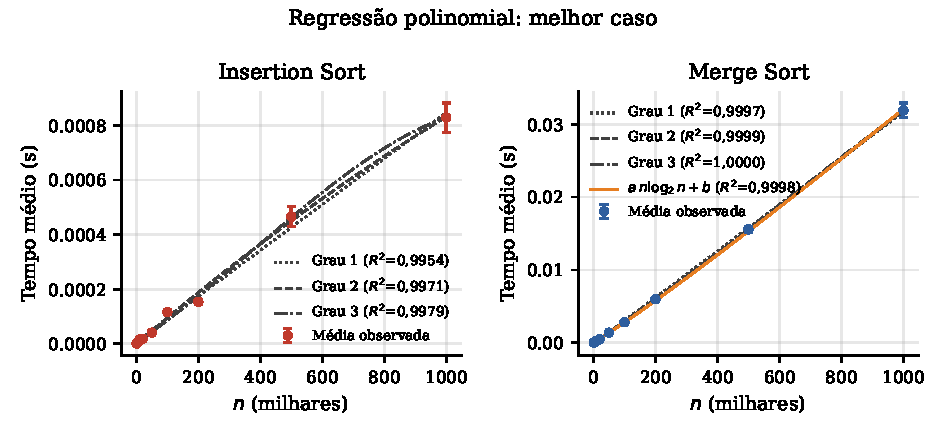
\includegraphics[width=\textwidth]{recursos/figuras/regressao_melhor.pdf}
    \fonte{Elaborada pelo autor (2026).}
\end{figure}

\begin{figure}[H]
    \caption{Médias observadas e curvas ajustadas no caso médio}
    \label{fig:reg-medio}
    \centering
    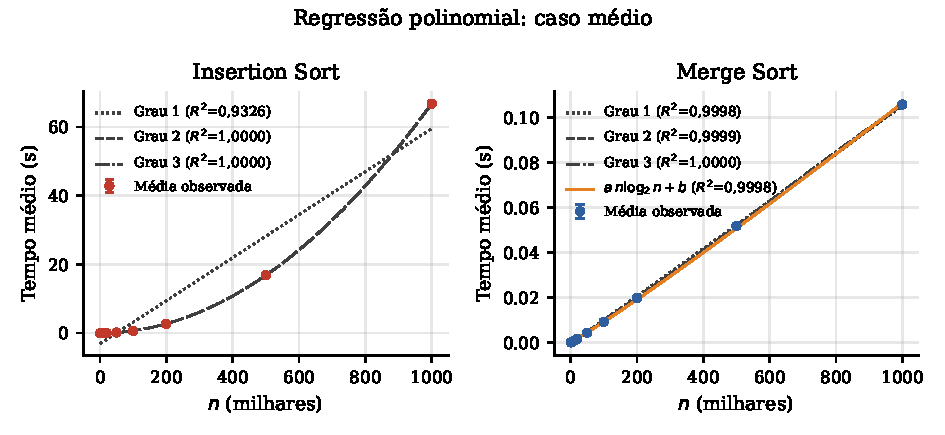
\includegraphics[width=\textwidth]{recursos/figuras/regressao_medio.pdf}
    \fonte{Elaborada pelo autor (2026).}
\end{figure}

\begin{figure}[H]
    \caption{Médias observadas e curvas ajustadas no pior caso}
    \label{fig:reg-pior}
    \centering
    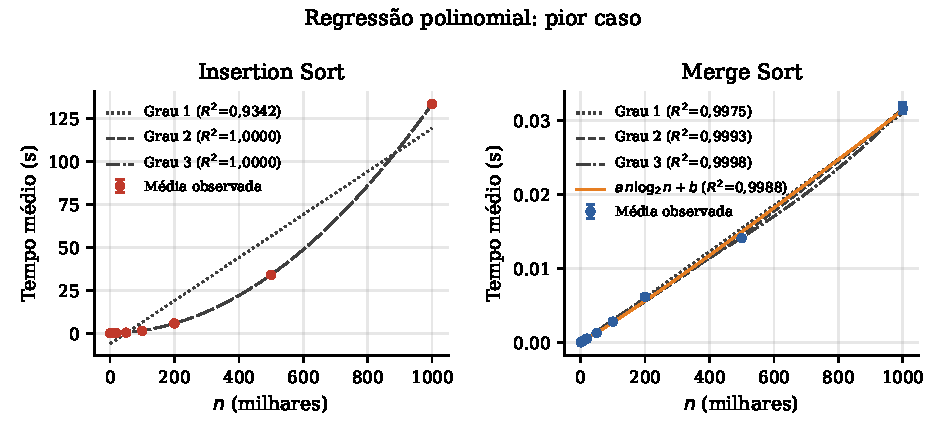
\includegraphics[width=\textwidth]{recursos/figuras/regressao_pior.pdf}
    \fonte{Elaborada pelo autor (2026).}
\end{figure}

\subsection{Insertion Sort}

Nos casos médio e pior, o polinômio de grau 1 teve ajuste ruim ($R^2$ de 0,933 e 0,934), enquanto o de grau 2 se ajustou quase perfeitamente ($R^2$ de 0,999999 e 0,9999996). As funções obtidas foram:

\begin{align*}
    T_{\text{médio}}(n) &\approx \num{6.635e-11}\, n^2 + \num{4.951e-7}\, n - \num{9.743e-3} \\
    T_{\text{pior}}(n)  &\approx \num{1.331e-10}\, n^2 + \num{1.322e-7}\, n + \num{1.612e-3}
\end{align*}

Essas funções têm a forma quadrática $T(n) = a n^2 + b n + c$ prevista pela teoria para o Insertion Sort \cite{cormen2012}, e o termo quadrático domina: com $n = \num{1000000}$, ele responde por mais de 99\,\% do valor da função. Os coeficientes também têm interpretação física. O coeficiente quadrático do pior caso ($\num{1.331e-10}$) é 2,01 vezes o do caso médio ($\num{6.635e-11}$), exatamente a razão entre $n^2/2$ e $n^2/4$ deslocamentos esperada pela contagem de inversões \cite{knuth1998}. Dividindo o tempo do caso médio com $n = \num{1000000}$ pelo número esperado de deslocamentos ($n^2/4$), obtém-se cerca de 0,27\,ns por deslocamento, o custo de uma iteração do laço interno nesta máquina. Os coeficientes linear e constante são pequenos, e o termo constante negativo do caso médio não tem significado físico: é apenas um artefato do ajuste, irrelevante diante do termo quadrático.

No melhor caso, o polinômio de grau 1, $T(n) \approx \num{8.413e-10}\, n + \num{5.975e-6}$, já se ajustou bem ($R^2 = 0{,}9954$). Isso é compatível com o comportamento linear previsto, a cerca de 0,8\,ns por elemento. Os graus 2 e 3 aumentaram o $R^2$ apenas marginalmente (para 0,9971 e 0,9979), e o termo de maior grau ficou negativo nos dois casos, o que não tem significado físico para um tempo de execução: é típico de um ajuste que passa a acompanhar o ruído das medições, e não uma tendência real.

O polinômio de grau 3 tem $R^2$ igual ou maior que o de grau 2 em todos os casos, por exemplo 1,000000 contra 0,999999 no caso médio. Isso, porém, não significa que o algoritmo tenha ordem de crescimento cúbica. Polinômios de grau maior contêm os de grau menor como caso particular: basta zerar o coeficiente adicional. Por isso, o ajuste por mínimos quadrados nunca piora quando se aumenta o grau, porque o termo extra sempre pode absorver parte do ruído. Com apenas dez pontos, um polinômio de grau suficientemente alto passaria exatamente por todos eles. O critério para escolher o modelo não deve ser apenas o maior $R^2$, e sim o menor grau que explica os dados com coeficientes coerentes. No Insertion Sort, o coeficiente cúbico obtido é desprezível e de sinal negativo ($-\num{1.146e-18}$ no caso médio), e o coeficiente quadrático praticamente não muda em relação ao ajuste de grau 2 ($\num{6.796e-11}$ contra $\num{6.635e-11}$). Isso mostra que o termo cúbico não representa uma tendência real dos dados. Portanto, o grau que melhor descreve o Insertion Sort é 2 nos casos médio e pior, e 1 no melhor caso, em concordância com a teoria.

\subsection{Merge Sort}

Para o Merge Sort, todos os modelos obtiveram $R^2$ acima de 0,999, inclusive o de grau 1. No caso médio, o polinômio de grau 1 ($R^2 = 0{,}99975$) e o modelo $n \log_2 n$ ($R^2 = 0{,}99975$) tiveram ajustes praticamente idênticos:

\begin{align*}
    T_{\text{médio}}(n) &\approx \num{1.058e-7}\, n - \num{5.772e-4} && \text{(grau 1)} \\
    T_{\text{médio}}(n) &\approx \num{5.322e-9}\, n \log_2 n + \num{3.056e-4} && (n \log_2 n)
\end{align*}

O polinômio de grau 2 melhorou um pouco o ajuste ($R^2 = 0{,}99992$), com coeficiente quadrático positivo e muito pequeno ($\num{5.350e-15}$). Esse termo não indica crescimento quadrático: ele aproxima a leve curvatura para cima que o fator $\log n$ produz em relação a uma reta. Com $n = \num{1000000}$, o termo quadrático corresponde a cerca de 5\,\% do valor da função, enquanto no Insertion Sort o termo quadrático corresponde a quase todo o tempo.

A regressão polinomial é, portanto, consistente com o modelo teórico linearítmico. No entanto, nesse intervalo de tamanhos ela não consegue distinguir com clareza $n \log n$ de um crescimento linear. Como o fator $\log_2 n$ apenas dobra (de aproximadamente 10 para 20) enquanto $n$ é multiplicado por mil, as duas curvas são muito parecidas, e o ajuste por mínimos quadrados sobre as médias é dominado pelos maiores valores de $n$. No melhor caso, o modelo $n \log_2 n$ teve ajuste um pouco melhor que o linear ($R^2$ de 0,99981 contra 0,99972). No pior caso ocorreu o inverso (0,99906 contra 0,99986). As evidências mais claras do fator logarítmico são as razões ao dobrar $n$ ligeiramente acima de 2 (\autoref{sec:dobro}) e a grande diferença em relação ao comportamento quadrático do Insertion Sort, e não o $R^2$.

\pendente{revisar as funções e os valores de $R^2$ do pior caso após incluir $n = \num{1000000}$}

% ═══════════════════════════════════════════════════
\chapter{Conclusão}
\label{cap:conclusao}

O experimento confirmou empiricamente as ordens de crescimento previstas pela análise teórica. O Insertion Sort apresentou crescimento quadrático nos casos médio e pior, com expoentes empíricos de 1,96 e 1,97, razão próxima de 4 ao dobrar $n$ e polinômio de grau 2 com $R^2$ de 0,999999, e crescimento linear no melhor caso. O Merge Sort apresentou crescimento quase linear nos três cenários, com razão próxima de 2,1 ao dobrar $n$, compatível com $\Theta(n \log n)$. A relação de 2 entre os coeficientes quadráticos do pior caso e do caso médio do Insertion Sort coincidiu com a razão entre os números de inversões dos vetores decrescente e aleatório, o que mostra que a regressão capturou não apenas a forma da função, mas também a contagem de operações que a teoria descreve.

Na comparação entre os algoritmos, o Merge Sort foi significativamente mais rápido em todos os tamanhos testados nos casos médio e pior, com uma vantagem que cresceu de 1,3 vez com $n = \num{1000}$ para mais de 600 vezes com $n = \num{1000000}$ no caso médio. O Insertion Sort, por sua vez, foi de 17 a 39 vezes mais rápido no melhor caso. Esses resultados mostram que a escolha do algoritmo depende do tamanho e da configuração da entrada, e não apenas da ordem de crescimento.

O experimento também evidenciou o que a análise assintótica deixa de fora: as constantes multiplicativas, que tornam o Insertion Sort competitivo em entradas pequenas; a influência da configuração da entrada nas constantes do Merge Sort, cujo caso médio foi cerca de 3,3 vezes mais lento que os demais apesar da mesma ordem de crescimento; e a variabilidade das medições, que exigiu repetições e intervalos de confiança para que as conclusões fossem confiáveis. Também mostrou um limite do método: no intervalo estudado, o $R^2$ da regressão não foi suficiente para distinguir $n \log n$ de crescimento linear, e indicadores como a razão ao dobrar $n$ e o expoente empírico foram mais informativos. A análise teórica prevê como o custo cresce, e a análise empírica mostra quanto esse custo vale na prática e a partir de que ponto as previsões se tornam visíveis. As duas são complementares.

Como trabalhos futuros, sugere-se medir tamanhos abaixo de \num{1000} para localizar o ponto de cruzamento entre os algoritmos no caso médio e contar comparações e movimentações, além do tempo, para verificar as explicações propostas para as diferenças entre cenários do Merge Sort.

\pendente{revisar a conclusão após incluir o pior caso com $n = \num{1000000}$}

% ─── PÓS-TEXTUAIS ──────────────────────────────────
\postextual

\emreferenciastrue
\bibliography{referencias}
\emreferenciasfalse

\begin{apendicesenv}
\partapendices

\chapter{Reprodução do experimento}
\label{apendice:reproducao}

Os comandos a seguir, executados na raiz do projeto, reproduzem o ciclo completo de compilação, execução, análise e geração deste relatório.

\begin{lstlisting}[language=bash]
# 1. Compilar e executar o benchmark (grava os CSVs em resultados/)
make
./main

# 2. Preparar o ambiente Python e gerar tabelas e figuras
python3 -m venv venv
venv/bin/pip install -r requirements.txt
venv/bin/python analise.py                # saídas em saida/
venv/bin/python docs/gerar_recursos.py    # saídas em docs/recursos/

# 3. Compilar o relatório
cd docs && latexmk -pdf relatorio.tex
\end{lstlisting}

Os algoritmos, cenários e tamanhos executados pelo benchmark são definidos no bloco de configuração no início do arquivo \texttt{main.c}, pelos vetores \texttt{algoritmos\_a\_rodar}, \texttt{cenarios\_a\_rodar} e \texttt{tamanhos\_a\_rodar}. Cada execução sobrescreve apenas os arquivos das combinações selecionadas.

\end{apendicesenv}

\end{document}
